\documentclass[../../main.tex]{subfiles}
\graphicspath{{\subfix{../../image/}}} % 指定图片目录,后续可以直接使用图片文件名。

% 例如:
% \begin{figure}[H]
% \centering
% \includegraphics[scale=0.4]{图.png}
% \caption{}
% \label{figure:图}
% \end{figure}
% 注意:上述\label{}一定要放在\caption{}之后,否则引用图片序号会只会显示??.

\begin{document}

\section{三次样条插值}

\begin{definition}[三次样条函数]
若函数 $S(x) \in C^2[a, b]$, 且在每个小区间 $[x_j, x_{j + 1}]$ 上是三次多项式, 其中 $a = x_0 < x_1 < \cdots < x_n = b$ 是给定节点, 则称 $S(x)$ 是节点 $x_0, x_1, \cdots, x_n$ 上的\textbf{三次样条函数}. 若在节点 $x_j$ 上给定函数值 $y_j = f(x_j)$ ($j = 0, 1, \cdots, n$), 并成立
\begin{align}
S(x_j) = y_j, \quad j = 0, 1, \cdots, n, \label{eq:数值分析-6.1}
\end{align}
则称 $S(x)$ 为\textbf{三次样条插值函数}.
\end{definition}
\begin{remark}
从定义知要求出 $S(x)$, 在每个小区间 $[x_j, x_{j + 1}]$ 上要确定 4 个待定系数, 而共有 $n$ 个小区间, 故应确定 $4n$ 个参数. 根据 $S(x)$ 在 $[a, b]$ 上二阶导数连续, 在节点 $x_j$ ($j = 1, 2, \cdots, n - 1$) 处应满足连续性条件
\begin{align}
S(x_j - 0) = S(x_j + 0), \quad S'(x_j - 0) = S'(x_j + 0), \quad S''(x_j - 0) = S''(x_j + 0). \label{eq:数值分析-6.2}
\end{align}
这里共有 $3n - 3$ 个条件, 再加上 $S(x)$ 满足插值条件 \eqref{eq:数值分析-6.1}, 共有 $4n - 2$ 个条件, 因此还需要加上 2 个条件才能确定 $S(x)$. 通常可在区间 $[a, b]$ 的端点 $a = x_0, b = x_n$ 上各加一个条件(称为边界条件), 可根据实际问题的要求给定. 常见的有以下 3 种:

(1) 已知两端的一阶导数值, 即
\begin{align}
S'(x_0) = f_0', \quad S'(x_n) = f_n'. \label{eq:数值分析-6.3}
\end{align}

(2) 两端的二阶导数已知, 即
\begin{align}
S''(x_0) = f_0'', \quad S''(x_n) = f_n'', \label{eq:数值分析-6.4}
\end{align}
其特殊情况为
\begin{align}
S''(x_0) = S''(x_n) = 0. \label{eq:数值分析-6.4'}
\end{align}
\eqref{eq:数值分析-6.4'} 式称为\textbf{自然边界条件}.

(3) 当 $f(x)$ 是以 $x_n - x_0$ 为周期的周期函数时, 则要求 $S(x)$ 也是周期函数. 这时边界条件应满足
\begin{align}
\begin{cases}
S(x_0 + 0) = S(x_n - 0), \, S'(x_0 + 0) = S'(x_n - 0), \\
S''(x_0 + 0) = S''(x_n - 0),
\end{cases} \label{eq:数值分析-6.5}
\end{align}
而此时 \eqref{eq:数值分析-6.1} 式中 $y_0 = y_n$. 这样确定的样条函数 $S(x)$ 称为\textbf{周期样条函数}.
\end{remark}

\vspace{0.5cm}

构造满足插值条件 \eqref{eq:数值分析-6.1} 及相应边界条件的三次样条插值函数 $S(x)$ 的表达式可以有多种方法. 例如,可以直接利用分段三次埃尔米特插值, 只要假定 $S'(x_j) = m_j$ ($j = 0, 1, \cdots, n$), 再由插值条件 \eqref{eq:数值分析-6.1} 可得
\begin{align}
S(x) = \sum_{j=0}^n [ y_j \alpha_j(x) + m_j \beta_j(x) ], \label{eq:数值分析-6.6}
\end{align}
其中 $\alpha_j(x), \beta_j(x)$ 是由 \eqref{eq:数值分析-4.8} 式~ \eqref{eq:数值分析-4.11} 式表示的插值基函数, 利用条件 \eqref{eq:数值分析-6.2} 式及相应边界条件 \eqref{eq:数值分析-6.3} 式~ \eqref{eq:数值分析-6.5} 式, 则可得到关于 $m_j$ ($j = 0, 1, \cdots, n$) 的三对角方程组, 求出 $m_j$ 则得到所求的三次样条函数 $S(x)$.

\begin{theorem}
若已知函数$f\in C^4[a,b]$在节点 $a = x_0 < x_1 < \cdots < x_n = b$ 上的函数值 $y_0, y_1, \cdots, y_n$, 记 $h_j = x_{j + 1} - x_j$, $h = \max\limits_j h_j$.记$S(x)$为$f(x)$的三次样条插值函数,且满足三种边界条件之一,即满足\eqref{eq:数值分析-6.3}式或\eqref{eq:数值分析-6.4}式或\eqref{eq:数值分析-6.5}式,则三次样条表达式为
\begin{align}
S(x) &= M_j \frac{(x_{j + 1} - x)^3}{6 h_j} + M_{j + 1} \frac{(x - x_j)^3}{6 h_j} + \left( y_j - \frac{M_j h_j^2}{6} \right) \frac{x_{j + 1} - x}{h_j} \nonumber \\
&\quad + \left( y_{j + 1} - \frac{M_{j + 1} h_j^2}{6} \right) \frac{x - x_j}{h_j}, \quad j = 0, 1, \cdots, n - 1. \label{eq:数值分析-6..8}
\end{align}
其中$M_j(j=0,1,\cdots,n)$满足三对角方程组\eqref{eq:数值分析-6.13}或\eqref{eq:数值分析-6.16}.
\begin{enumerate}[(1)]
\item 对第一种边界条件,即
\begin{align*}
S'(x_0) = f_0', \quad S'(x_n) = f_n'.
\end{align*}
令 $\lambda_0 = 1, d_0 = \frac{6}{h_0} (f[x_0, x_1] - f_0')$, $\mu_n = 1, d_n = \frac{6}{h_{n - 1}} (f_n' - f[x_{n - 1}, x_n])$,则$M_j(j=0,1,\cdots,n)$满足三对角方程组
\begin{align}
\begin{pmatrix}
2 & \lambda_0 \\
\mu_1 & 2 & \lambda_1 \\
& \ddots & \ddots & \ddots \\
& & \mu_{n - 1} & 2 & \lambda_{n - 1} \\
& & & \mu_n & 2
\end{pmatrix}
\begin{pmatrix}
M_0 \\
M_1 \\
\vdots \\
M_{n - 1} \\
M_n
\end{pmatrix}
=
\begin{pmatrix}
d_0 \\
d_1 \\
\vdots \\
d_{n - 1} \\
d_n
\end{pmatrix}. \label{eq:数值分析-6.13}
\end{align}

\item 对第二种边界条件,即
\begin{align*}
S''(x_0) = f_0'', \quad S''(x_n) = f_n'', 
\end{align*}
令 $\lambda_0 = \mu_n = 0, d_0 = 2 f_0'', d_n = 2 f_n''$, 则
$M_j(j=0,1,\cdots,n)$也满足三对角方程组\eqref{eq:数值分析-6.13}. 

\item 对第三种边界条件,即
\begin{align*}
\begin{cases}
S(x_0 + 0) = S(x_n - 0), \, S'(x_0 + 0) = S'(x_n - 0), \\
S''(x_0 + 0) = S''(x_n - 0),
\end{cases}
\end{align*}
令
\[
\lambda_n = \frac{h_0}{h_{n - 1} + h_0}, \quad \mu_n = 1 - \lambda_n = \frac{h_{n - 1}}{h_{n - 1} + h_0},
\]
\[
d_n = 6 \frac{f[x_0, x_1] - f[x_{n - 1}, x_n]}{h_0 + h_{n - 1}}.
\]
则$M_j(j=0,1,\cdots,n)$满足三对角方程组
\begin{align}
\begin{pmatrix}
2 & \lambda_1 & & & \mu_1 \\
\mu_2 & 2 & \lambda_2 & & \\
& \ddots & \ddots & \ddots & \\
& & \mu_{n - 1} & 2 & \lambda_{n - 1} \\
\lambda_n & & & \mu_n & 2
\end{pmatrix}
\begin{pmatrix}
M_1 \\
M_2 \\
\vdots \\
M_{n - 1} \\
M_n
\end{pmatrix}
=
\begin{pmatrix}
d_1 \\
d_2 \\
\vdots \\
d_{n - 1} \\
d_n
\end{pmatrix}. \label{eq:数值分析-6.16}
\end{align}
\end{enumerate}
\end{theorem}
\begin{proof}
假定$S(x)$ 的二阶导数值 $S''(x_j) = M_j$ ($j = 0, 1, \cdots, n$) 表达 $S(x)$. 由于 $S(x)$ 在区间 $[x_j, x_{j + 1}]$ 上是三次多项式, 故 $S''(x)$ 在 $[x_j, x_{j + 1}]$ 上是线性函数, 可表示为
\begin{align}
S''(x) = M_j \frac{x_{j + 1} - x}{h_j} + M_{j + 1} \frac{x - x_j}{h_j}. \label{eq:数值分析-6.7}
\end{align}
对 $S''(x)$ 积分两次并利用 $S(x_j) = y_j$ 及 $S(x_{j + 1}) = y_{j + 1}$, 可定出积分常数, 于是得三次样条表达式
\begin{align}
S(x) &= M_j \frac{(x_{j + 1} - x)^3}{6 h_j} + M_{j + 1} \frac{(x - x_j)^3}{6 h_j} + \left( y_j - \frac{M_j h_j^2}{6} \right) \frac{x_{j + 1} - x}{h_j} \nonumber \\
&\quad + \left( y_{j + 1} - \frac{M_{j + 1} h_j^2}{6} \right) \frac{x - x_j}{h_j}, \quad j = 0, 1, \cdots, n - 1. \label{eq:数值分析-6.8}
\end{align}
这里 $h_j=x_{j+1}-x_j$,$M_j$ ($j = 0, 1, \cdots, n$) 是未知的. 为了确定 $M_j$ ($j = 0, 1, \cdots, n$), 对 $S(x)$ 求导得
\begin{align}
S'(x) &= -M_j \frac{(x_{j + 1} - x)^2}{2 h_j} + M_{j + 1} \frac{(x - x_j)^2}{2 h_j} + \frac{y_{j + 1} - y_j}{h_j} - \frac{M_{j + 1} - M_j}{6} h_j; \label{eq:数值分析-6.9}
\end{align}
由此可求得
\[
S'(x_j + 0) = -\frac{h_j}{3} M_j - \frac{h_j}{6} M_{j + 1} + \frac{y_{j + 1} - y_j}{h_j}.
\]
类似地可求出 $S(x)$ 在区间 $[x_{j - 1}, x_j]$ 上的表达式, 进而得
\[
S'(x_j - 0) = \frac{h_{j - 1}}{6} M_{j - 1} + \frac{h_{j - 1}}{3} M_j + \frac{y_j - y_{j - 1}}{h_{j - 1}}.
\]
利用 $S'(x_j + 0) = S'(x_j - 0)$ 可得
\begin{align}
\mu_j M_{j - 1} + 2 M_j + \lambda_j M_{j + 1} = d_j, \quad j = 1, 2, \cdots, n - 1, \label{eq:数值分析-6.10}
\end{align}
其中
\[
\mu_j = \frac{h_{j - 1}}{h_{j - 1} + h_j}, \quad \lambda_j = \frac{h_j}{h_{j - 1} + h_j},
\]
\begin{align}
d_j = 6 \frac{f[x_j, x_{j + 1}] - f[x_{j - 1}, x_j]}{h_{j - 1} + h_j} = 6 f[x_{j - 1}, x_j, x_{j + 1}], \quad j = 1, 2, \cdots, n - 1. \label{eq:数值分析-6.11}
\end{align}

(1)对第一种边界条件 \eqref{eq:数值分析-6.3}, 可导出两个方程
\begin{align}
\begin{cases}
2 M_0 + M_1 = \frac{6}{h_0} (f[x_0, x_1] - f_0'), \\
M_{n - 1} + 2 M_n = \frac{6}{h_{n - 1}} (f_n' - f[x_{n - 1}, x_n]).
\end{cases} \label{eq:数值分析-6.12}
\end{align}
如果令 $\lambda_0 = 1, d_0 = \frac{6}{h_0} (f[x_0, x_1] - f_0')$, $\mu_n = 1, d_n = \frac{6}{h_{n - 1}} (f_n' - f[x_{n - 1}, x_n])$, 那么 \eqref{eq:数值分析-6.10} 式及 \eqref{eq:数值分析-6.12} 式可写成矩阵形式
\begin{align}
\begin{pmatrix}
2 & \lambda_0 \\
\mu_1 & 2 & \lambda_1 \\
& \ddots & \ddots & \ddots \\
& & \mu_{n - 1} & 2 & \lambda_{n - 1} \\
& & & \mu_n & 2
\end{pmatrix}
\begin{pmatrix}
M_0 \\
M_1 \\
\vdots \\
M_{n - 1} \\
M_n
\end{pmatrix}
=
\begin{pmatrix}
d_0 \\
d_1 \\
\vdots \\
d_{n - 1} \\
d_n
\end{pmatrix}. \label{eq:数值分析-6..13}
\end{align}

(2)对第二种边界条件 \eqref{eq:数值分析-6.4}, 直接得端点方程
\begin{align}
M_0 = f_0'', \quad M_n = f_n''. \label{eq:数值分析-6.14}
\end{align}
如果令 $\lambda_0 = \mu_n = 0, d_0 = 2 f_0'', d_n = 2 f_n''$, 则 \eqref{eq:数值分析-6.10} 式和 \eqref{eq:数值分析-6.14} 式也可以写成 \eqref{eq:数值分析-6..13} 式的形式.

(3)对于第三种边界条件 \eqref{eq:数值分析-6.5}, 可得
\begin{align}
M_0 = M_n, \quad \lambda_n M_1 + \mu_n M_{n - 1} + 2 M_n = d_n, \label{eq:数值分析-6.15}
\end{align}
其中
\[
\lambda_n = \frac{h_0}{h_{n - 1} + h_0}, \quad \mu_n = 1 - \lambda_n = \frac{h_{n - 1}}{h_{n - 1} + h_0},
\]
\[
d_n = 6 \frac{f[x_0, x_1] - f[x_{n - 1}, x_n]}{h_0 + h_{n - 1}}.
\]
\eqref{eq:数值分析-6.10} 式和 \eqref{eq:数值分析-6.15} 式可以写成矩阵形式
\begin{align}
\begin{pmatrix}
2 & \lambda_1 & & & \mu_1 \\
\mu_2 & 2 & \lambda_2 & & \\
& \ddots & \ddots & \ddots & \\
& & \mu_{n - 1} & 2 & \lambda_{n - 1} \\
\lambda_n & & & \mu_n & 2
\end{pmatrix}
\begin{pmatrix}
M_1 \\
M_2 \\
\vdots \\
M_{n - 1} \\
M_n
\end{pmatrix}
=
\begin{pmatrix}
d_1 \\
d_2 \\
\vdots \\
d_{n - 1} \\
d_n
\end{pmatrix}. \label{eq:数值分析-6..16}
\end{align}

\end{proof}
\begin{remark}
线性方程组 \eqref{eq:数值分析-6..13} 和 \eqref{eq:数值分析-6..16} 是关于 $M_j$ ($j = 0, 1, \cdots, n$) 的三对角线性方程组, $M_j$ 在力学上解释为细梁在 $x_j$ 截面处的弯矩, 称为 $S(x)$ 的矩, 线性方程组 \eqref{eq:数值分析-6..13} 和 \eqref{eq:数值分析-6..16} 称为三弯矩方程. 方程组 \eqref{eq:数值分析-6..13} 和 \eqref{eq:数值分析-6..16} 的系数矩阵中元素 $\lambda_j, \mu_j$ 已完全确定. 并且满足 $\lambda_j \geqslant 0, \mu_j \geqslant 0, \lambda_j + \mu_j = 1$. 因此系数矩阵为严格对角占优阵, 从而方程组 \eqref{eq:数值分析-6..13} 和 \eqref{eq:数值分析-6..16} 有唯一解. 求解方法可见 5.3 节追赶法, 将解得结果代入 \eqref{eq:数值分析-6..8} 式即可.
\end{remark}

\begin{theorem}\label{theorem:数值分析-定理-5}
设 $f(x)\in C^4[a,b]$,$S(x)$ 为满足第一种或第二种边界条件\eqref{eq:数值分析-6.3}或\eqref{eq:数值分析-6.4}的三次样条函数,令 $h=\max\limits_{0\leqslant i\leqslant n-1} h_i$,$h_i=x_{i+1}-x_i$($i=0,1,\cdots,n-1$),则有估计式
\begin{align}\label{eq:数值分析-6.17}
\max\limits_{a\leqslant x\leqslant b} | f^{(k)}(x) - S^{(k)}(x) | \leqslant C_k \max\limits_{a\leqslant x\leqslant b} | f^{(4)}(x) | h^{4-k}, \quad k = 0,1,2,
\end{align}
其中 $C_0=\frac{5}{384}$,$C_1=\frac{1}{24}$,$C_2=\frac{3}{8}$。
\end{theorem}
\begin{note}
这个定理不但给出了三次样条插值函数 $S(x)$ 的误差估计,而且说明当 $h\to 0$ 时,$S(x)$ 及其一阶导数 $S'(x)$ 和二阶导数 $S''(x)$ 均分别一致收敛于 $f(x)$,$f'(x)$ 及 $f''(x)$。
\end{note}
\begin{proof}


\end{proof}

\begin{example}
设 $f(x)$ 为定义在 $[27.7,30]$ 上的函数,在节点 $x_i$($i=0,1,2,3$)上的值如下:
$$f(x_0)=f(27.7)=4.1, \quad f(x_1)=f(28)=4.3,$$
$$f(x_2)=f(29)=4.1, \quad f(x_3)=f(30)=3.0.$$
试求三次样条函数 $S(x)$,使它满足边界条件 $S'(27.7)=3.0$,$S'(30)=-4.0$。
\end{example}
\begin{solution}
先由 \eqref{eq:数值分析-6.11}式及 \eqref{eq:数值分析-6.12}式计算 $h_0=0.30$,$h_1=h_2=1$,$\mu_1=\frac{3}{13}$,$\mu_2=\frac{1}{2}$,$\mu_3=1$,$\lambda_0=1$,$\lambda_1=\frac{10}{13}$,$\lambda_2=\frac{1}{2}$,$d_0=\frac{6}{h_0}(f[x_0,x_1]-f'_0)=-46.666$,$d_1=6f[x_0,x_1,x_2]=-4.00002$,$d_2=6f[x_1,x_2,x_3]=-2.70000$,$d_3=\frac{6}{h_2}(f'_3-f[x_2,x_3])=-17.4$。
由此得矩阵形式的线性方程组 (6.13) 为
$$\begin{pmatrix}
2 & 1 & & \\
\frac{3}{13} & 2 & \frac{10}{13} & \\
& \frac{1}{2} & 2 & \frac{1}{2} \\
& & 1 & 2
\end{pmatrix}
\begin{pmatrix}
M_0 \\
M_1 \\
M_2 \\
M_3
\end{pmatrix}
=
\begin{pmatrix}
-46.6666 \\
-4.00002 \\
-2.7000 \\
-17.4000
\end{pmatrix}.$$
求解此方程组得到
$$M_0=-23.531, \quad M_1=0.396,$$
$$M_2=0.830, \quad M_3=-9.115.$$
将 $M_0,M_1,M_2,M_3$ 代入表达式 \eqref{eq:数值分析-6.8}得到(曲线见\reffig{figure:三次样条插值例题7})。
\begin{figure}[H]
\centering
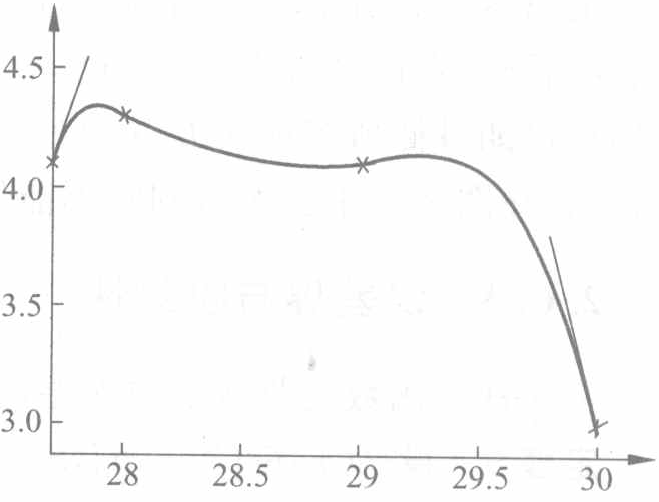
\includegraphics[scale=0.3]{三次样条插值例题7.png}
\caption{}
\label{figure:三次样条插值例题7}
\end{figure}
$$
S(x)=
\begin{cases}
13.07278(x-28)^3 - 14.84322(x-28) + 0.22000(x-27.7)^3 + 14.31353(x-27.7), & x \in [27.7,28], \\
0.06600(29-x)^3 + 4.23400(29-x) + 0.13833(x-28)^3 + 3.96167(x-28), & x \in [28,29], \\
0.13833(30-x)^3 + 3.96167(30-x) - 1.51917(x-29)^3 + 4.51917(x-29), & x \in [29,30].
\end{cases}
$$
通常求三次样条函数可根据上述例题的计算步骤直接编程上机计算,或直接使用数学库中的软件,根据具体要求算出结果即可。

\end{solution}

\begin{example}
给定函数 $f(x)=\frac{1}{1+x^2}$,$-5\leqslant x\leqslant 5$,节点 $x_k=-5+k$($k=0,1,\cdots,10$),求三次样条插值 $S_{10}(x)$。
\end{example}
\begin{solution}
\begin{table}[H]
\centering
\caption{}
\label{table:数值分析例题表格2-7}
\begin{tabular}{c c c c || c c c c}
\hline
$x$ & $\frac{1}{1+x^2}$ & $S_{10}(x)$ & $L_{10}(x)$ & $x$ & $\frac{1}{1+x^2}$ & $S_{10}(x)$ & $L_{10}(x)$ \\
\hline
$-5.0$ & $0.038\ 46$ & $0.038\ 46$ & $0.038\ 46$ & $-2.3$ & $0.158\ 98$ & $0.161\ 15$ & $0.241\ 45$ \\
$-4.8$ & $0.041\ 60$ & $0.037\ 58$ & $1.804\ 38$ & $-2.0$ & $0.200\ 00$ & $0.200\ 00$ & $0.200\ 00$ \\
$-4.5$ & $0.047\ 06$ & $0.042\ 48$ & $1.578\ 72$ & $-1.8$ & $0.235\ 85$ & $0.231\ 54$ & $0.188\ 78$ \\
$-4.3$ & $0.051\ 31$ & $0.048\ 42$ & $0.888\ 08$ & $-1.5$ & $0.307\ 69$ & $0.297\ 44$ & $0.235\ 35$ \\
$-4.0$ & $0.058\ 82$ & $0.058\ 82$ & $0.058\ 82$ & $-1.3$ & $0.371\ 75$ & $0.361\ 33$ & $0.316\ 50$ \\
$-3.8$ & $0.064\ 77$ & $0.065\ 56$ & $-0.201\ 30$ & $-1.0$ & $0.500\ 00$ & $0.500\ 00$ & $0.500\ 00$ \\
$-3.5$ & $0.075\ 47$ & $0.076\ 06$ & $-0.226\ 20$ & $-0.8$ & $0.609\ 76$ & $0.624\ 20$ & $0.643\ 16$ \\
$-3.3$ & $0.084\ 10$ & $0.084\ 26$ & $-0.108\ 32$ & $-0.5$ & $0.800\ 00$ & $0.820\ 51$ & $0.843\ 40$ \\
$-3.0$ & $0.100\ 00$ & $0.100\ 00$ & $0.100\ 00$ & $-0.3$ & $0.917\ 43$ & $0.927\ 54$ & $0.940\ 90$ \\
$-2.8$ & $0.113\ 12$ & $0.113\ 66$ & $0.198\ 37$ & $0$ & $1.000\ 00$ & $1.000\ 00$ & $1.000\ 00$ \\
$-2.5$ & $0.137\ 93$ & $0.139\ 71$ & $0.253\ 76$ &  &  &  &  \\
\hline
\end{tabular}
\end{table}
取 $S_{10}(x_k)=f(x_k)$($k=0,1,\cdots,10$),$S'_{10}(-5)=f'(-5)$,$S'_{10}(5)=f'(5)$。直接上机计算可求出 $S_{10}(x)$ 在\reftab{table:数值分析例题表格2-7} 所列各点的值(利用对称性,这里只列出在负半轴上各点的值)。从表中看到,在所列各点 $S_{10}(x)$ 与 $f(x)$ 误差较小,它可作为 $f(x)$ 在区间 $[-5,5]$ 上的近似,而用拉格朗日插值多项式 $L_{10}(x)$ 计算相应点上的值 $L_{10}(x)$(也见\reftab{table:数值分析例题表格2-7}),显然它与 $f(x)$ 相差很大,在\reffig{figure:高次插值的龙格现象}中已经看到它不能作为 $f(x)$ 的近似。

\end{solution}

















\end{document}